\documentclass{article}
\usepackage[margin=1in]{geometry}
\usepackage{graphicx}
\usepackage{caption}
\usepackage{subcaption}
\graphicspath{{../screenshots}}
\usepackage{xeCJK}
\setCJKmainfont{Noto Serif CJK TC}

\renewcommand{\familydefault}{\sfdefault}
\title{Networks Systems Capstone Lab 3 Report}
\author{Andr\'es Ponce \
\and
彭思安
}
\begin{document}
\maketitle
\section{Part 1}
\subsection{Take a screenshot of the routing tables before/after on [r1-r4].}

\begin{figure}[h]
	%\label{fig:RoutingTables}
	\centering
	\begin{subfigure}{0.5\textwidth}
		\centering
		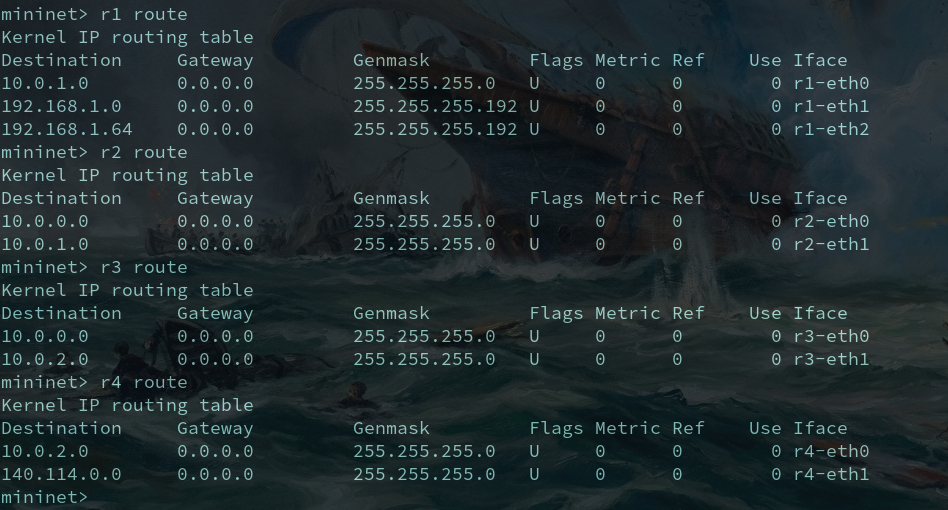
\includegraphics[scale=0.2]{1RoutingBefore.png}
		\caption{Routing tables before turning on BGP daemon.}
	\end{subfigure}%
	\begin{subfigure}{0.5\textwidth}
		\centering
		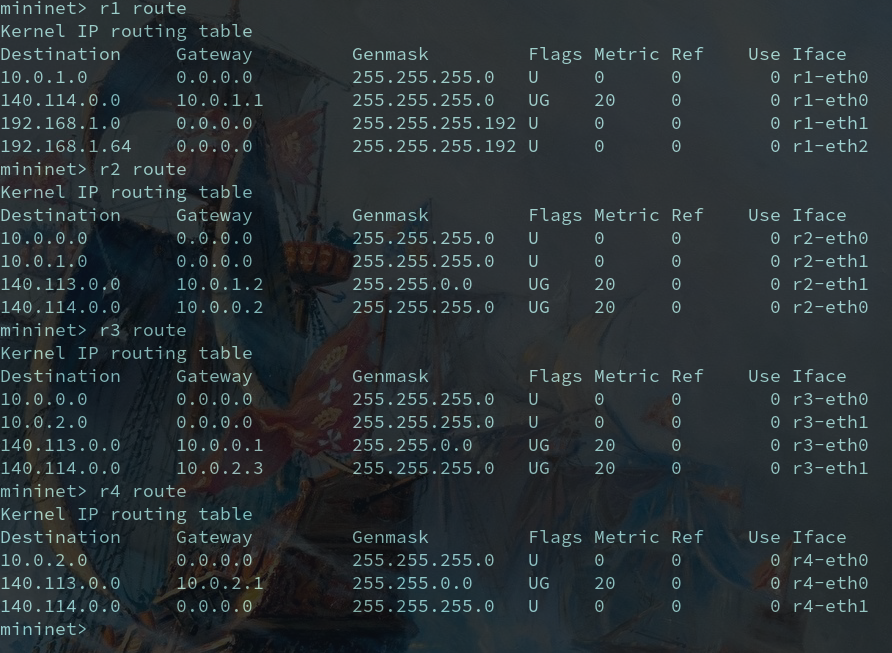
\includegraphics[scale=0.2]{2RoutingAfter.png}
		\caption{Routing tables after turning on the BGP daemon.}
	\end{subfigure}
	\caption{Routing tables of each router.}
\end{figure}
When the BGP daemon starts the routes will be added to the routing tables of each router.

\subsection{Telnet zebra and bgpd daemons of [r1-r4] and take screenshots of routes in zebra
and bgpd daemons.}

\subsection{Capture BGP packets from wireshark and take screenshots to verify your answer
to the following questions.}


\subsubsection{Show BGP packets exchanged by r2 and r3.}

\begin{figure}
	\label{fig:BGPMessages}
	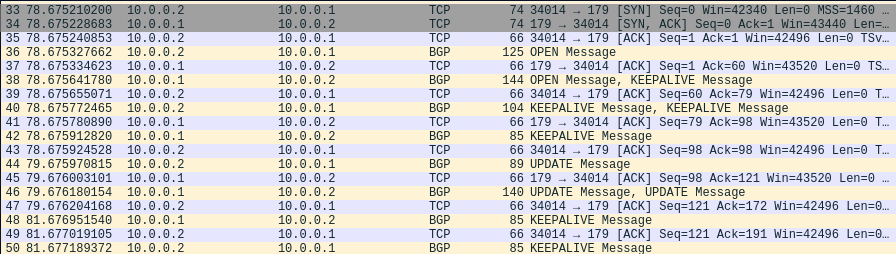
\includegraphics[scale=0.3]{3BGPMessages.png}
	\caption{OPEN, UPDATE, KEEPALIVE messages exchanged by r2 and r3.}
\end{figure}

\subsubsection{What will happen to the routing table if you set r4-eth0 down?}
If we set r4 down, its address will be flushed from the other routers.

\subsubsection{How does r3 know that r4 is unreachable? Explain how.}
As part of the BGP settings, we set the \texttt{timers connect 5} option for each neighbor.
A timer counts from zero to the amount of seconds specifiied in the configuration file.
If a Keepalive message is not received within that time, that peer information is flushed
from the neighbor's routing table.
This means that BGP will flush any neighbors who for some reason become inactive for 
a certain time.
Since r3 fails to receive a Keepalive message form r4 when the timer reaches zero, 
r3 assumes that the neighbor is dead.

\subsubsection{How does r2 know that r4 is unreachable? Explain how.}
Now that r3 knows that r4 is inactive, it will broadcast that message around the network.
When r2 receives information that r4 is inactive, it will also drop flush that route
and advertise the message to the other routers.

\section{Part 2}
\subsection{Explain the difference in packet headers.}
Once the iptable rules have been set, the information in each packet that goes through
the router will have its source or destination changed depending on the rule it matches.
The DNAT rule will work whenever we want to access the HTTP server at the given port.
Likewise for the SNAT will match any packet coming in from the given subnet, and then
the router will change the source field to its own address.
\end{document}

